\chapter{Alternative detection techniques}
\section{Subspace Detection}
Although not incorporated into the results presented in the preceding chapters, we have developed and implemented functionality for additional detection techniques not detailed above. Specifically, we have developed functionality for the use of `subspace detection' of repeating and near-repeating seismicity, which we summarize below.

Matched-filter detection techniques are computationally expensive when applied
across large datasets. The expense is multiplied as more earthquakes are added
to the list of template events (referred to by \citet{Barrett_2014} as a `design set') and as larger seismograph networks with more channels of data are used. At the same time, it is important that a set of template events effectively represent the variety of sources present in a given study area or risk missing what might be important seismicity. Subspace detection has been used to address these considerations by expressing clusters of similar events as single matrices known as subspace detectors \citep[for example][]{Harris_2006a,Harris_2006, Barrett_2014,Chambers_2015}.

\subsection{Subspace detector design}
As outlined by \citet{Harris_2006a}, there are five main steps in constructing a series of subspace detectors from a catalog of earthquakes:
\begin{enumerate}
    \item Generate a distance matrix for all events by calculating, pairwise, the correlations between events in the catalog. Each element of the distance matrix, $D_{x, y}$ is equivalent to $1 - R(x, y)$ where $R(x, y)$ is the cross correlation value between events $x$ and $y$;
    \item Cluster the events in the catalog based on this distance matrix. \citet{Harris_2006a} suggest a single-link agglomerative hierarchical clustering algorithm. Each cluster is then referred to as the design set for a single subspace detector;
    \item For each cluster, align the waveforms by cross correlation and trim the waveforms such that the first arrival occurs at the same point for each trace. Each waveform defines a column, $i$, of the data vector, $\underline{X}$;
    \item Calculate the orthonormal basis, $\underline{W}$, for the space defined by the design set, $\underline{X}$:

    \begin{equation}
    \underline{X} = \underline{W} \underline{\Sigma} \underline{V}^{T}
    \end{equation}
    
    \item Determine a satisfactory dimension $d$ such that the subspace defined by $\underline{W}_{d}$ approximates the waveforms in the design set:
    
    \begin{equation}
    \underline{X} \sim \underline{W}_{d} \underline{\Sigma}_{d} \underline{V}_{d}^{T}
    \end{equation}
    
    $W_{d}$ is our subspace detector and the matrix:
    
    \begin{equation}
    \underline{A}_{d} = \underline{\Sigma}_{d}\underline{V}_{d}^{T}
    \end{equation}
    
    gives the relative importance of each dimension, $d$, of $\underline{W}_{d}$ in describing the design set, $\underline{X}$.
\end{enumerate}

\subsection{Detection statistic}
Following the notation above, the detection statistic is defined as the following:

\begin{equation}
c[n] = \frac{\underline{x}_{p}^{T}[n]\underline{x}_{p}[n]}{\underline{x}^{T}[n]\underline{x}[n]}
\end{equation}

where $\underline{x}[n]$ is the data vector within the moving detection window and $\underline{x}_{p}[n]$ is the projection of $\underline{x}[n]$ onto the space defined by the subspace detector such that:

\begin{equation}
\underline{x}_{p}[n] = \underline{W}_{d}\underline{W}_{d}^{T}\underline{x}[n]
\end{equation}

This defines the ratio of the energy in the projected data $x_{p}[n]$ to the energy in the original data, $x[n]$ within the detection window $[n]$, which moves through the data period of interest one sample at a time.

\subsection{Determining a sufficient dimension}
Typically, the necessary number of dimensions in a subspace detector is determined empirically, using a plot such as Figure \ref{425783}, which shows the percentage of energy captured by the detector for all design set events with increasing dimensionality. For instance, \citet{Chambers_2015} stipulate that the desired dimension, $d$, is the smallest dimension for which the subspace detector, $\underline{W}_{d}$ captures an average of 90\% of the energy for all events in the design set, $\underline{X}$.\selectlanguage{english}

\begin{figure}[h!]
\begin{center}
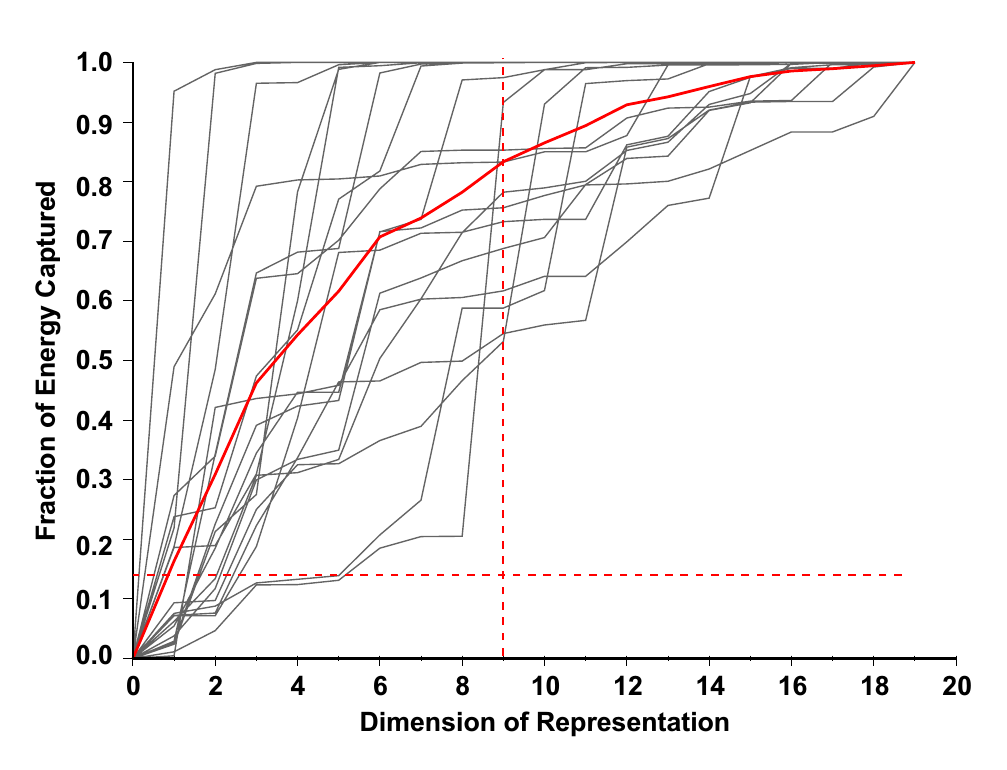
\includegraphics[width=0.70\columnwidth]{Appendices/EQcorrscan/figures/Harris_2006_fig8/Harris_2006_fig8}
\caption[Energy capture of subspace detectors with dimension]{{Adapted from Harris et al. (2006), showing the percentage energy capture
by a subspace detector with increasing dimensionality. Gray lines show
energy capture for each event in the design set used to construct the
detector and the solid red line shows the average across all events. The
dotted red lines indicate the dimension (n=9) corresponding to an
average energy capture of 90\%.
{\label{425783}}%
}}
\end{center}
\end{figure}

\section{\textit{EQcorrscan} development}
The functionality detailed above encompasses my contribution to the open-source Python package, \textit{EQcorrscan} \citep{Chamberlain_2017b}, which is developed and maintained by VUW postdoctoral fellow Calum Chamberlain. The purpose of \textit{EQcorrscan} is to provide an easy-to-use, fully tested framework for the detection of repeating and near-repeating seismicity. The original development of the package centered around the matched-filter detection routine detailed in Chapter 2 but was expanded to include subspace detection during the course of this thesis.